\documentclass[a5paper]{scrartcl}
\usepackage{testpiece}
\usepackage{eso-pic}
\usepackage[left=0.5cm, right=0.5cm, bottom=0.5cm, top=4.75cm]{geometry}
\usepackage{multicol}
\usepackage{enumitem}
\setmainfont{Tex Gyre Schola}

\RedeclareSectionCommand[
  runin=false,
  beforeskip=0.0\baselineskip,
  afterskip=0.25\baselineskip
]{section}

\setkomafont{section}{\setmainfont[Scale=1.125]{Tex Gyre Schola}\LARGE\color{redfabric}\bfseries\scshape}

\begin{document}
\AddToShipoutPictureBG{
\begin{tikzpicture}[remember picture, overlay]
%	\node () at (current page.center) {\includegraphics[width=\pagewidth, height=\pageheight]{Images/aloft_cover_background.png}};
	\node () at (current page.center) {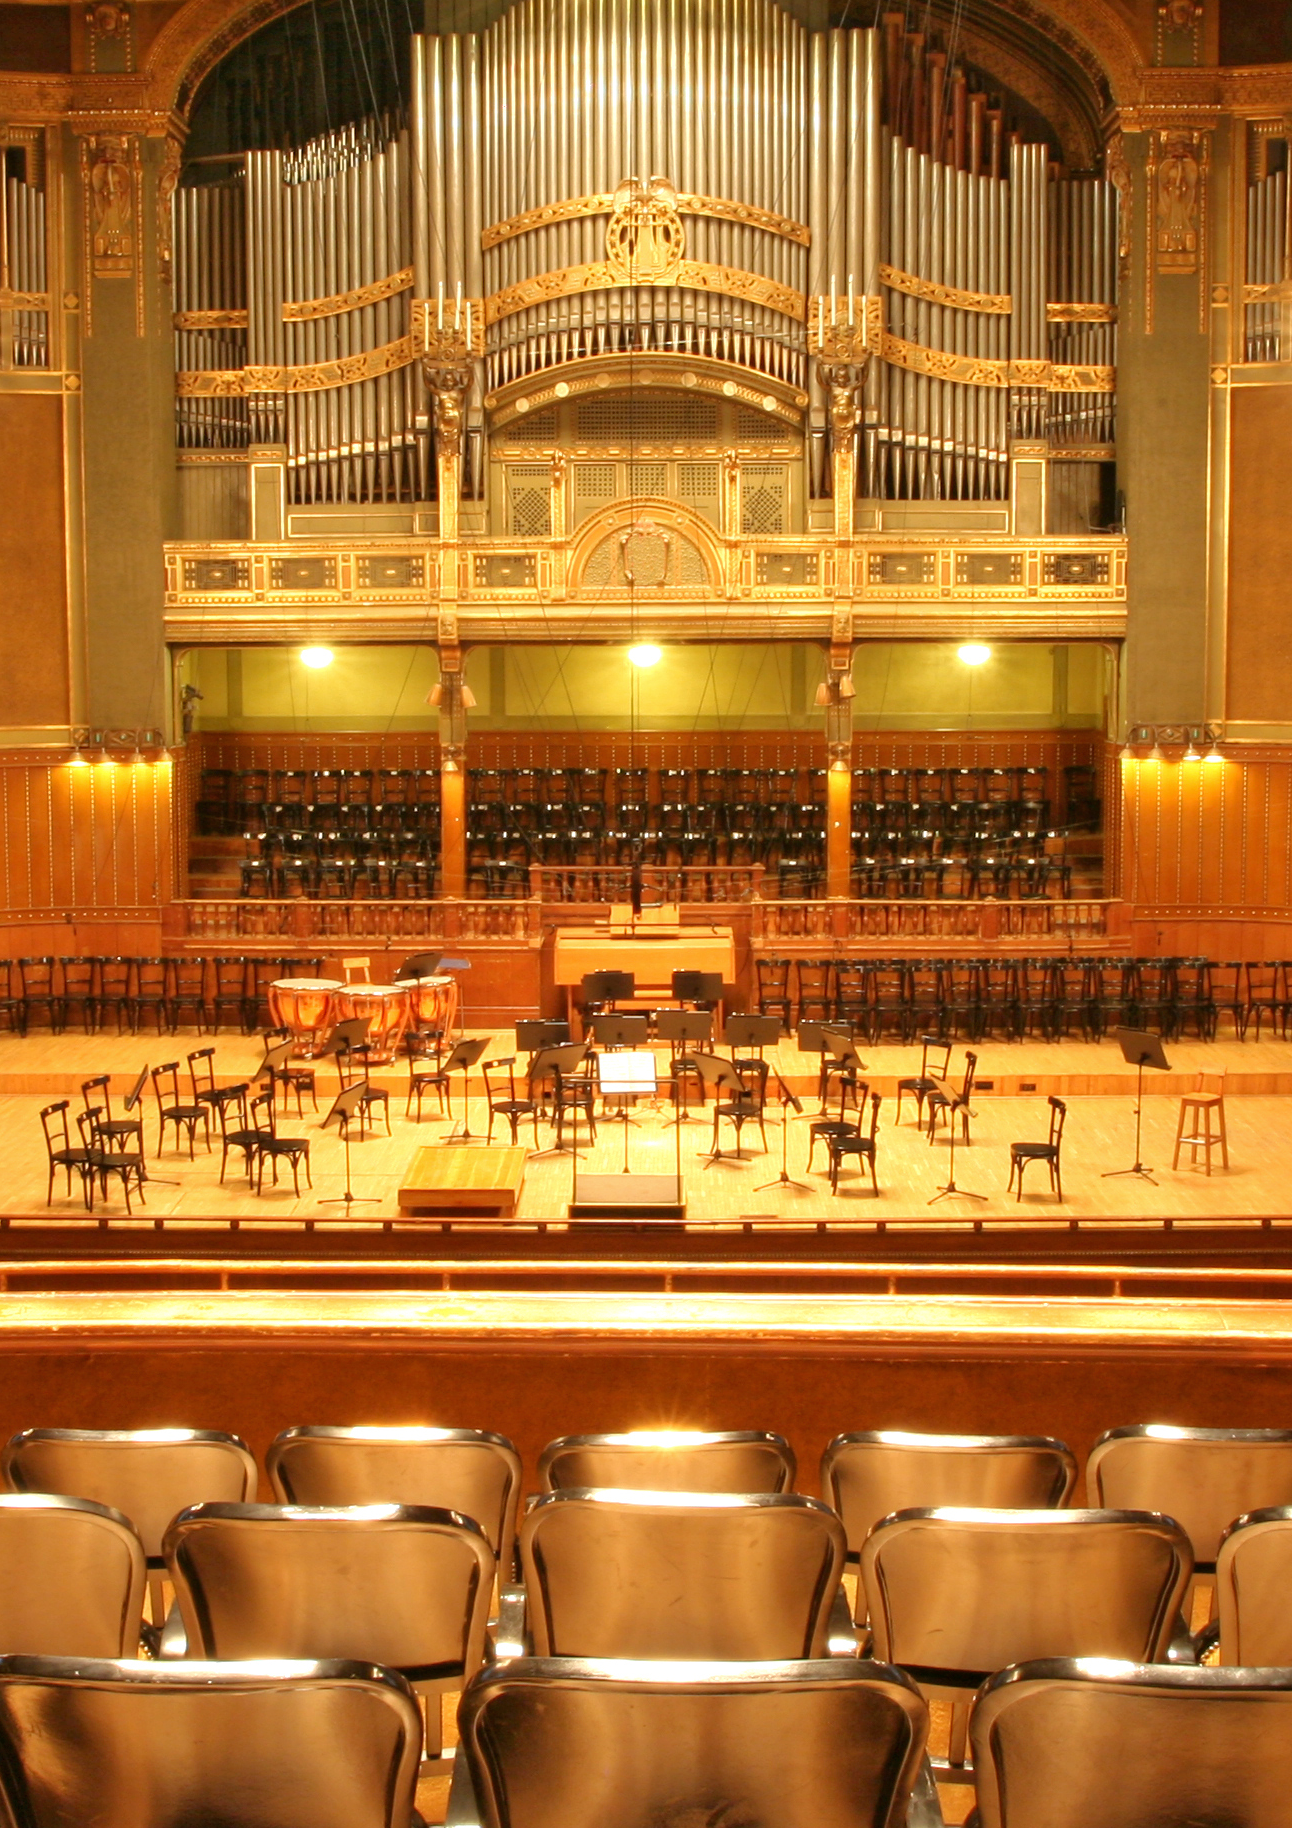
\includegraphics[width=\pagewidth, height=\pageheight]{Images/test_piece_front_cover_background.png}};
	\path (current page.north) --++ (0, -0.5cm) node[anchor=north] (banner) {
\includegraphics[width=\pagewidth]{Images/test_piece_banner.png}};
%	\path (current page.south) --++ (0, 0.5cm) node[fill=white, minimum height=160mm, minimum width=138.5mm, fill opacity=0.9, anchor=south] {};
\end{tikzpicture}
}
\raggedright

\begin{tikzpicture}
\node[text width=127.5mm, inner sep=5mm, draw, line width=0.5mm, fill=white, fill opacity=0.9, rounded corners=1mm] (a) at (0,0) {\vspace{-2ex}\section*{Overview} A two-player card-drafting game about brass bands. During the game, players assume the roles of rival music directors who are competing to build the best band from a limited pool of local musicians.
};

\path (a.south west) --++ (0, -0.5cm) node[draw, line width=0.5mm, text width=62mm, inner sep=5mm, fill=white, fill opacity=0.9, rounded corners=1mm, anchor=north west] (b) {\vspace{-2ex}\section*{Components} 36 cards, 8 pawns, 2 score boards.};

%\path (b.south) --++ (0cm, -3.25cm) node[rotate=0, transform shape] {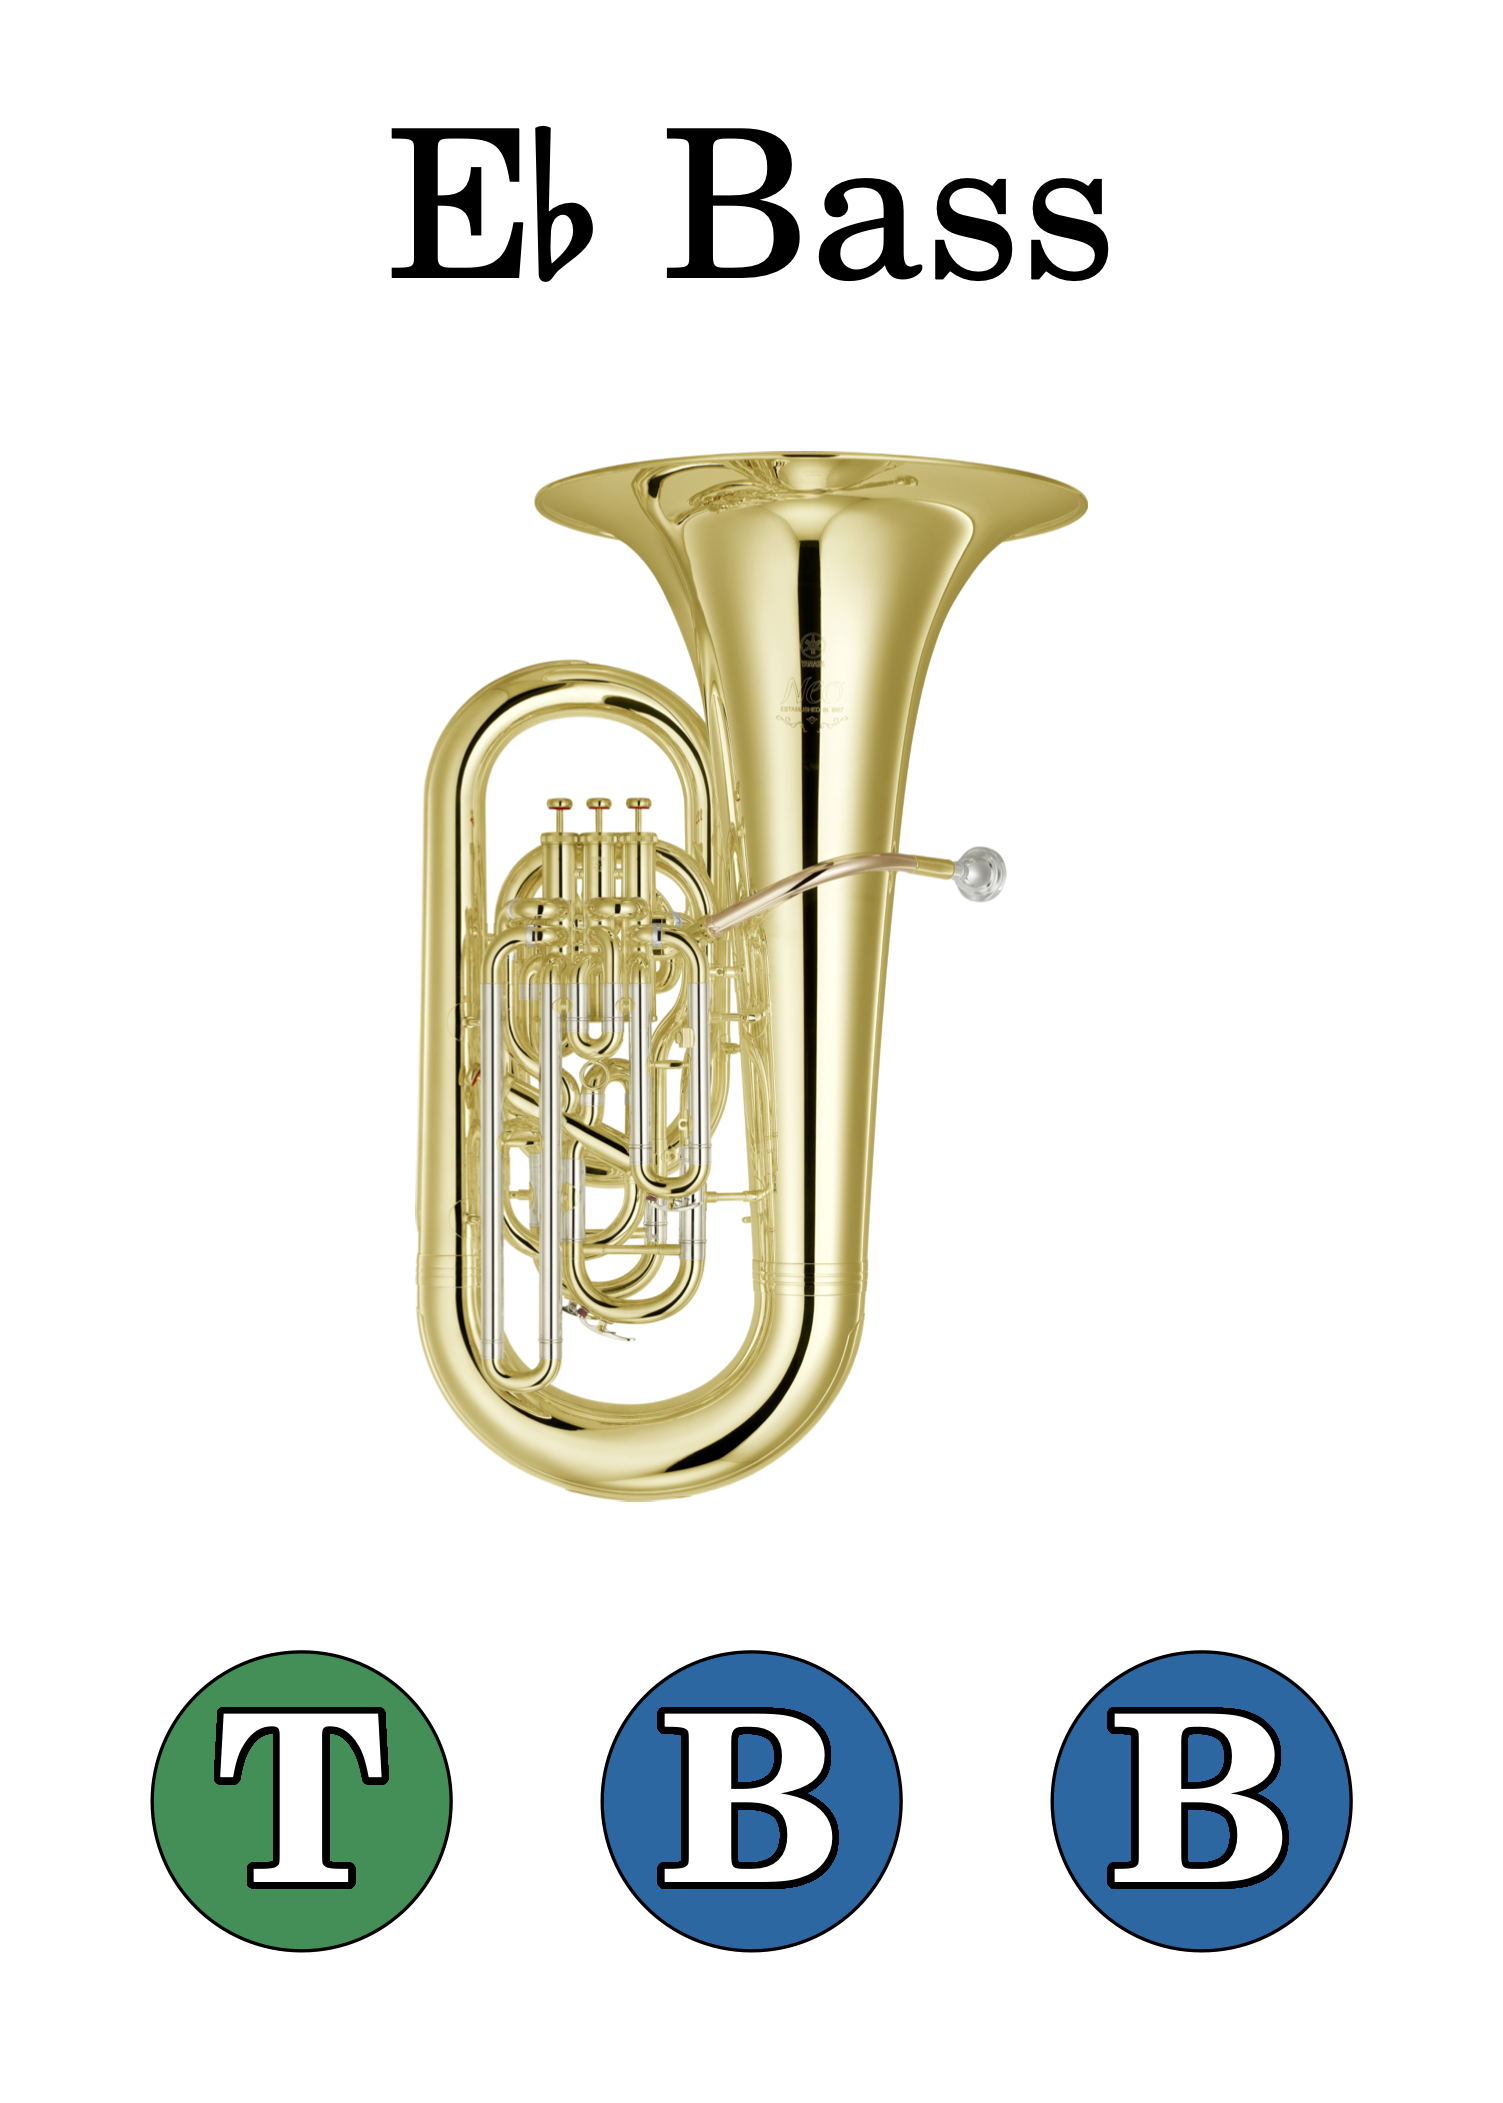
\includegraphics[height=3.5cm]{Images/CardImages/eflat_bass_card_front.png}};
\path (b.south west) --++ (-0.0cm, -1.3cm) node[anchor=north west, rotate=20, transform shape, inner sep=0pt] (cornet) {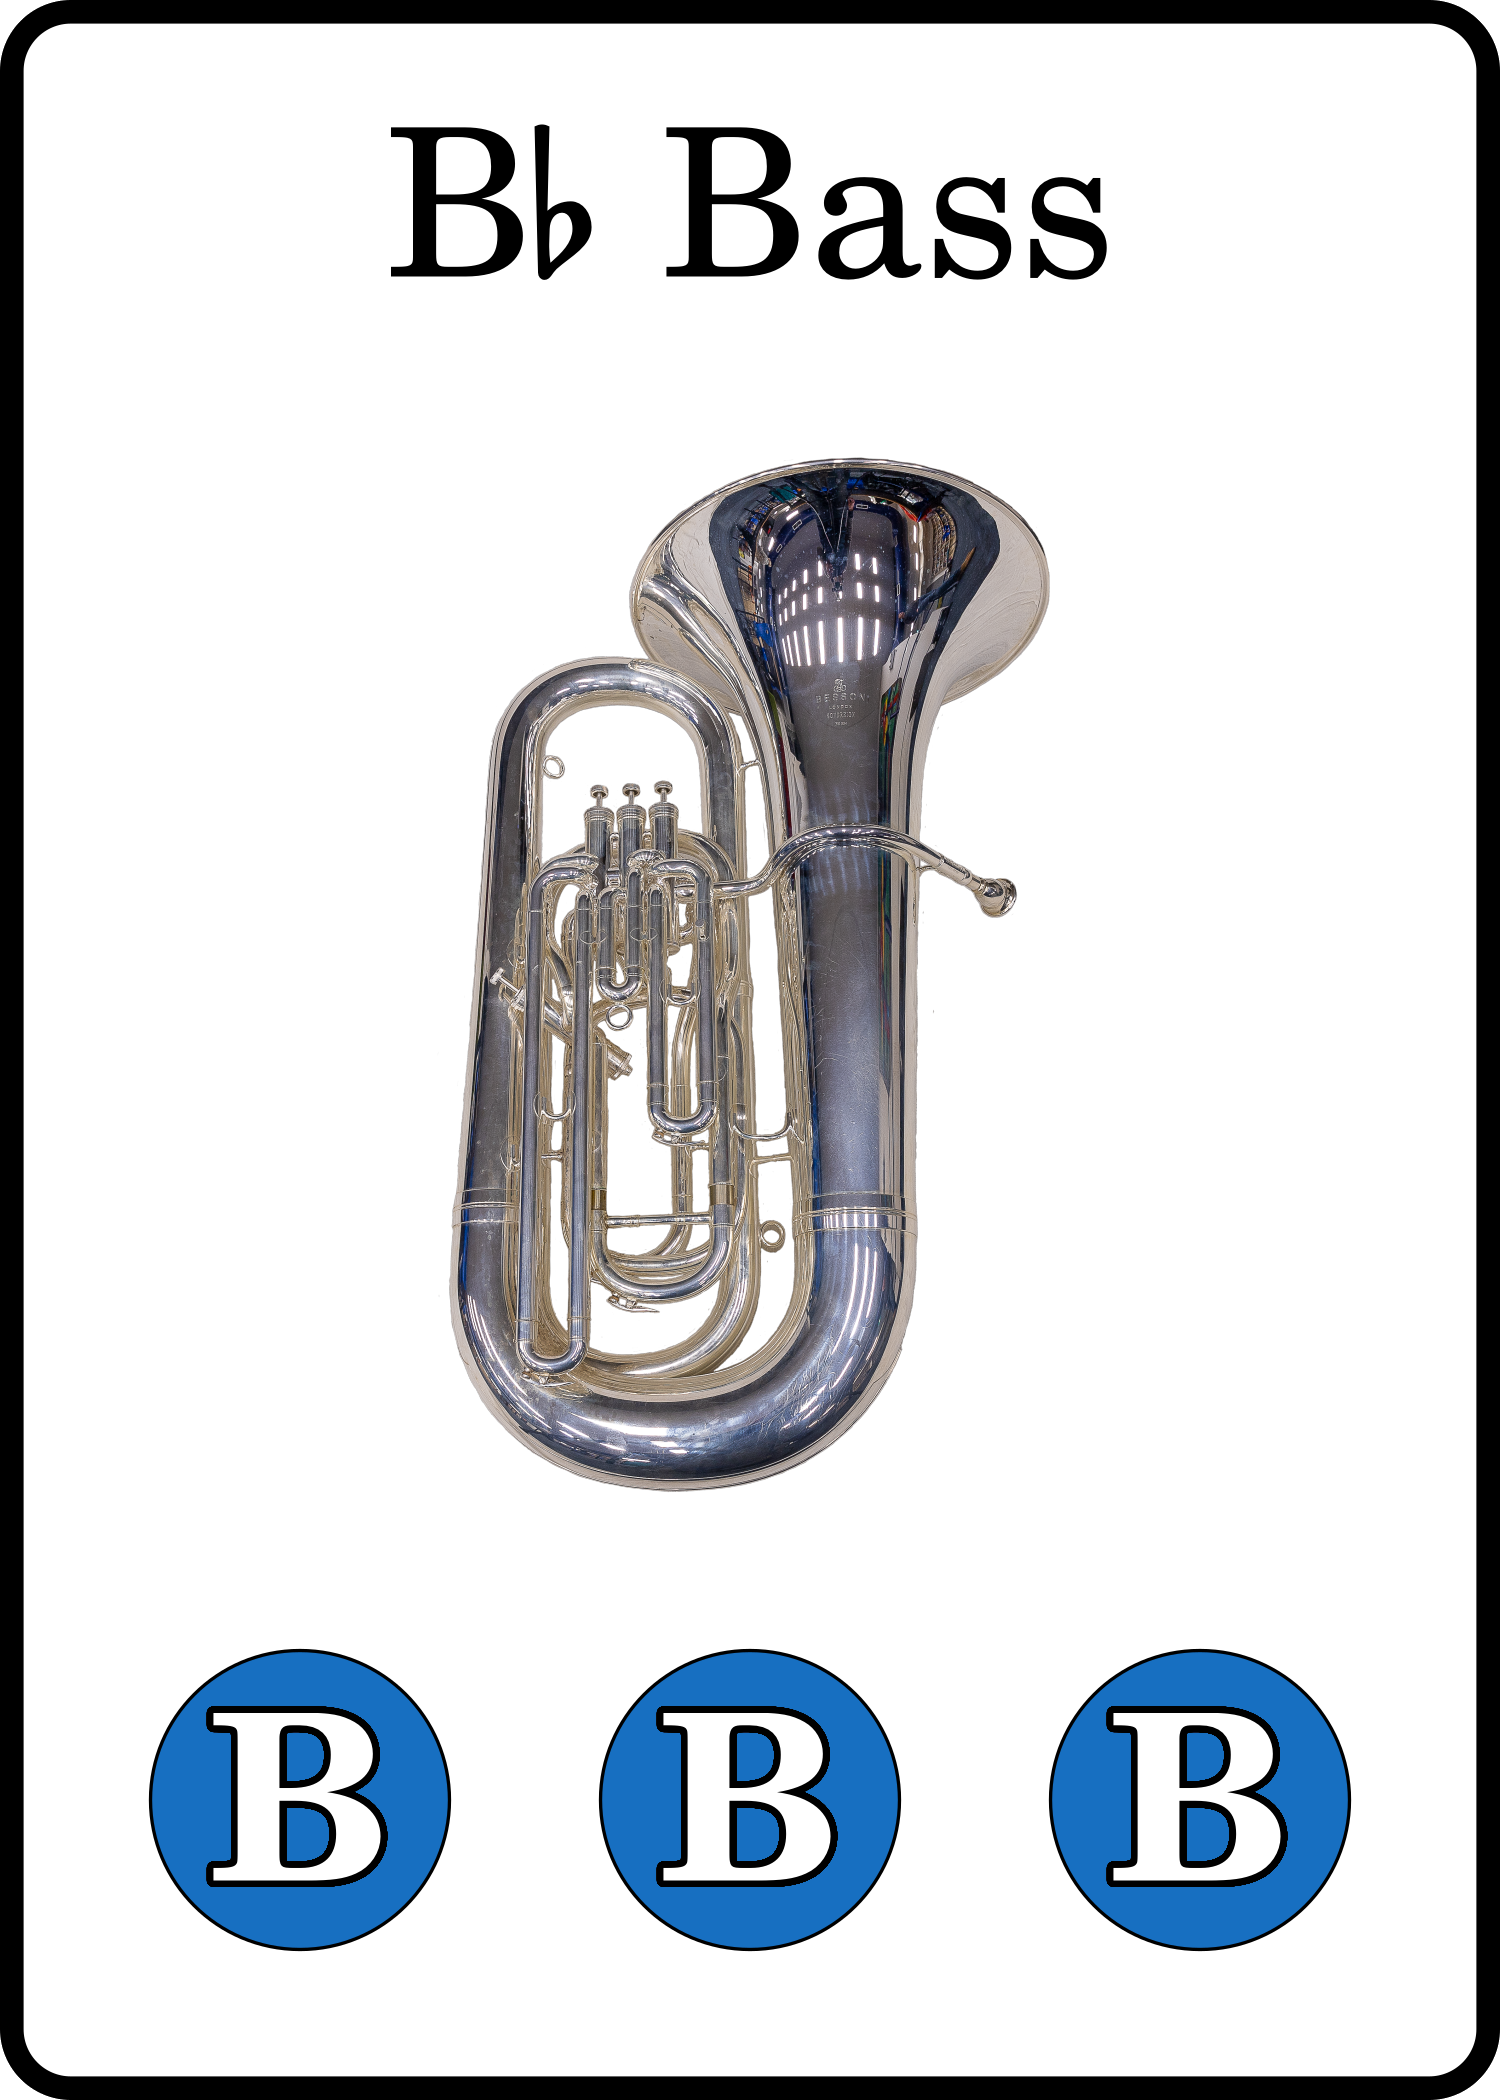
\includegraphics[height=3.75cm]{Images/CardImages/bass_display_front.png}};
\path (b.south) --++ (0cm, -0.45cm) node[anchor=north, rotate=0, transform shape, inner sep=0pt] (cornet) {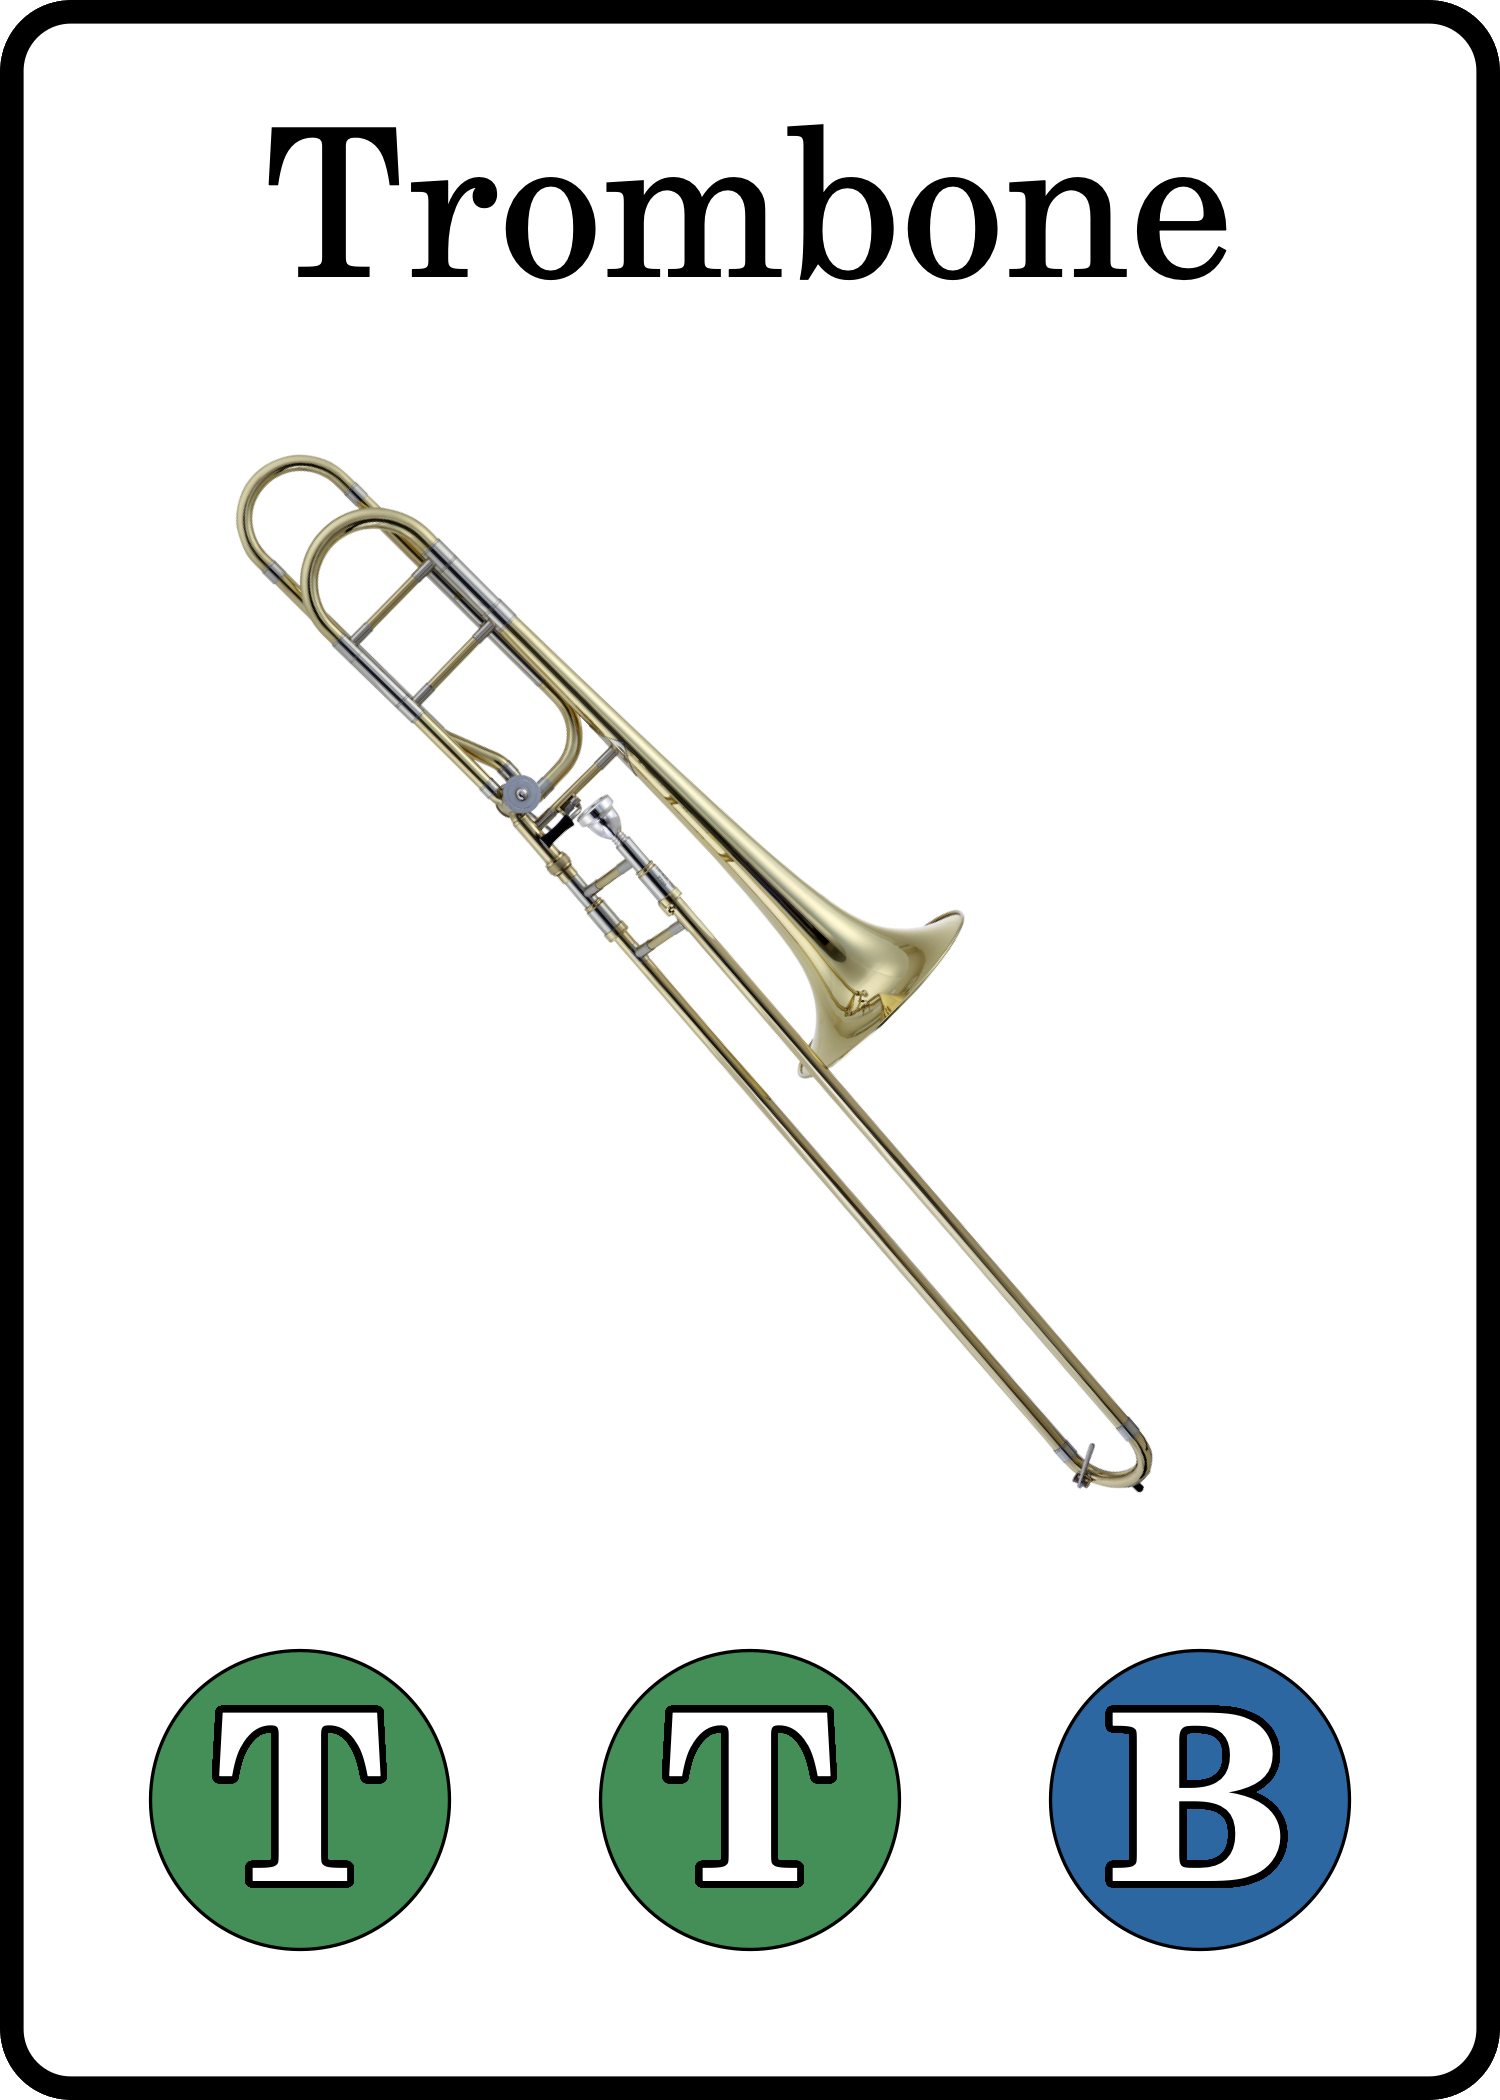
\includegraphics[height=3.75cm]{Images/CardImages/trombone_display_front.png}};
\path (b.south east) --++ (0.0cm, -1.3cm) node[anchor=north east, rotate=-20, transform shape, inner sep=0pt] {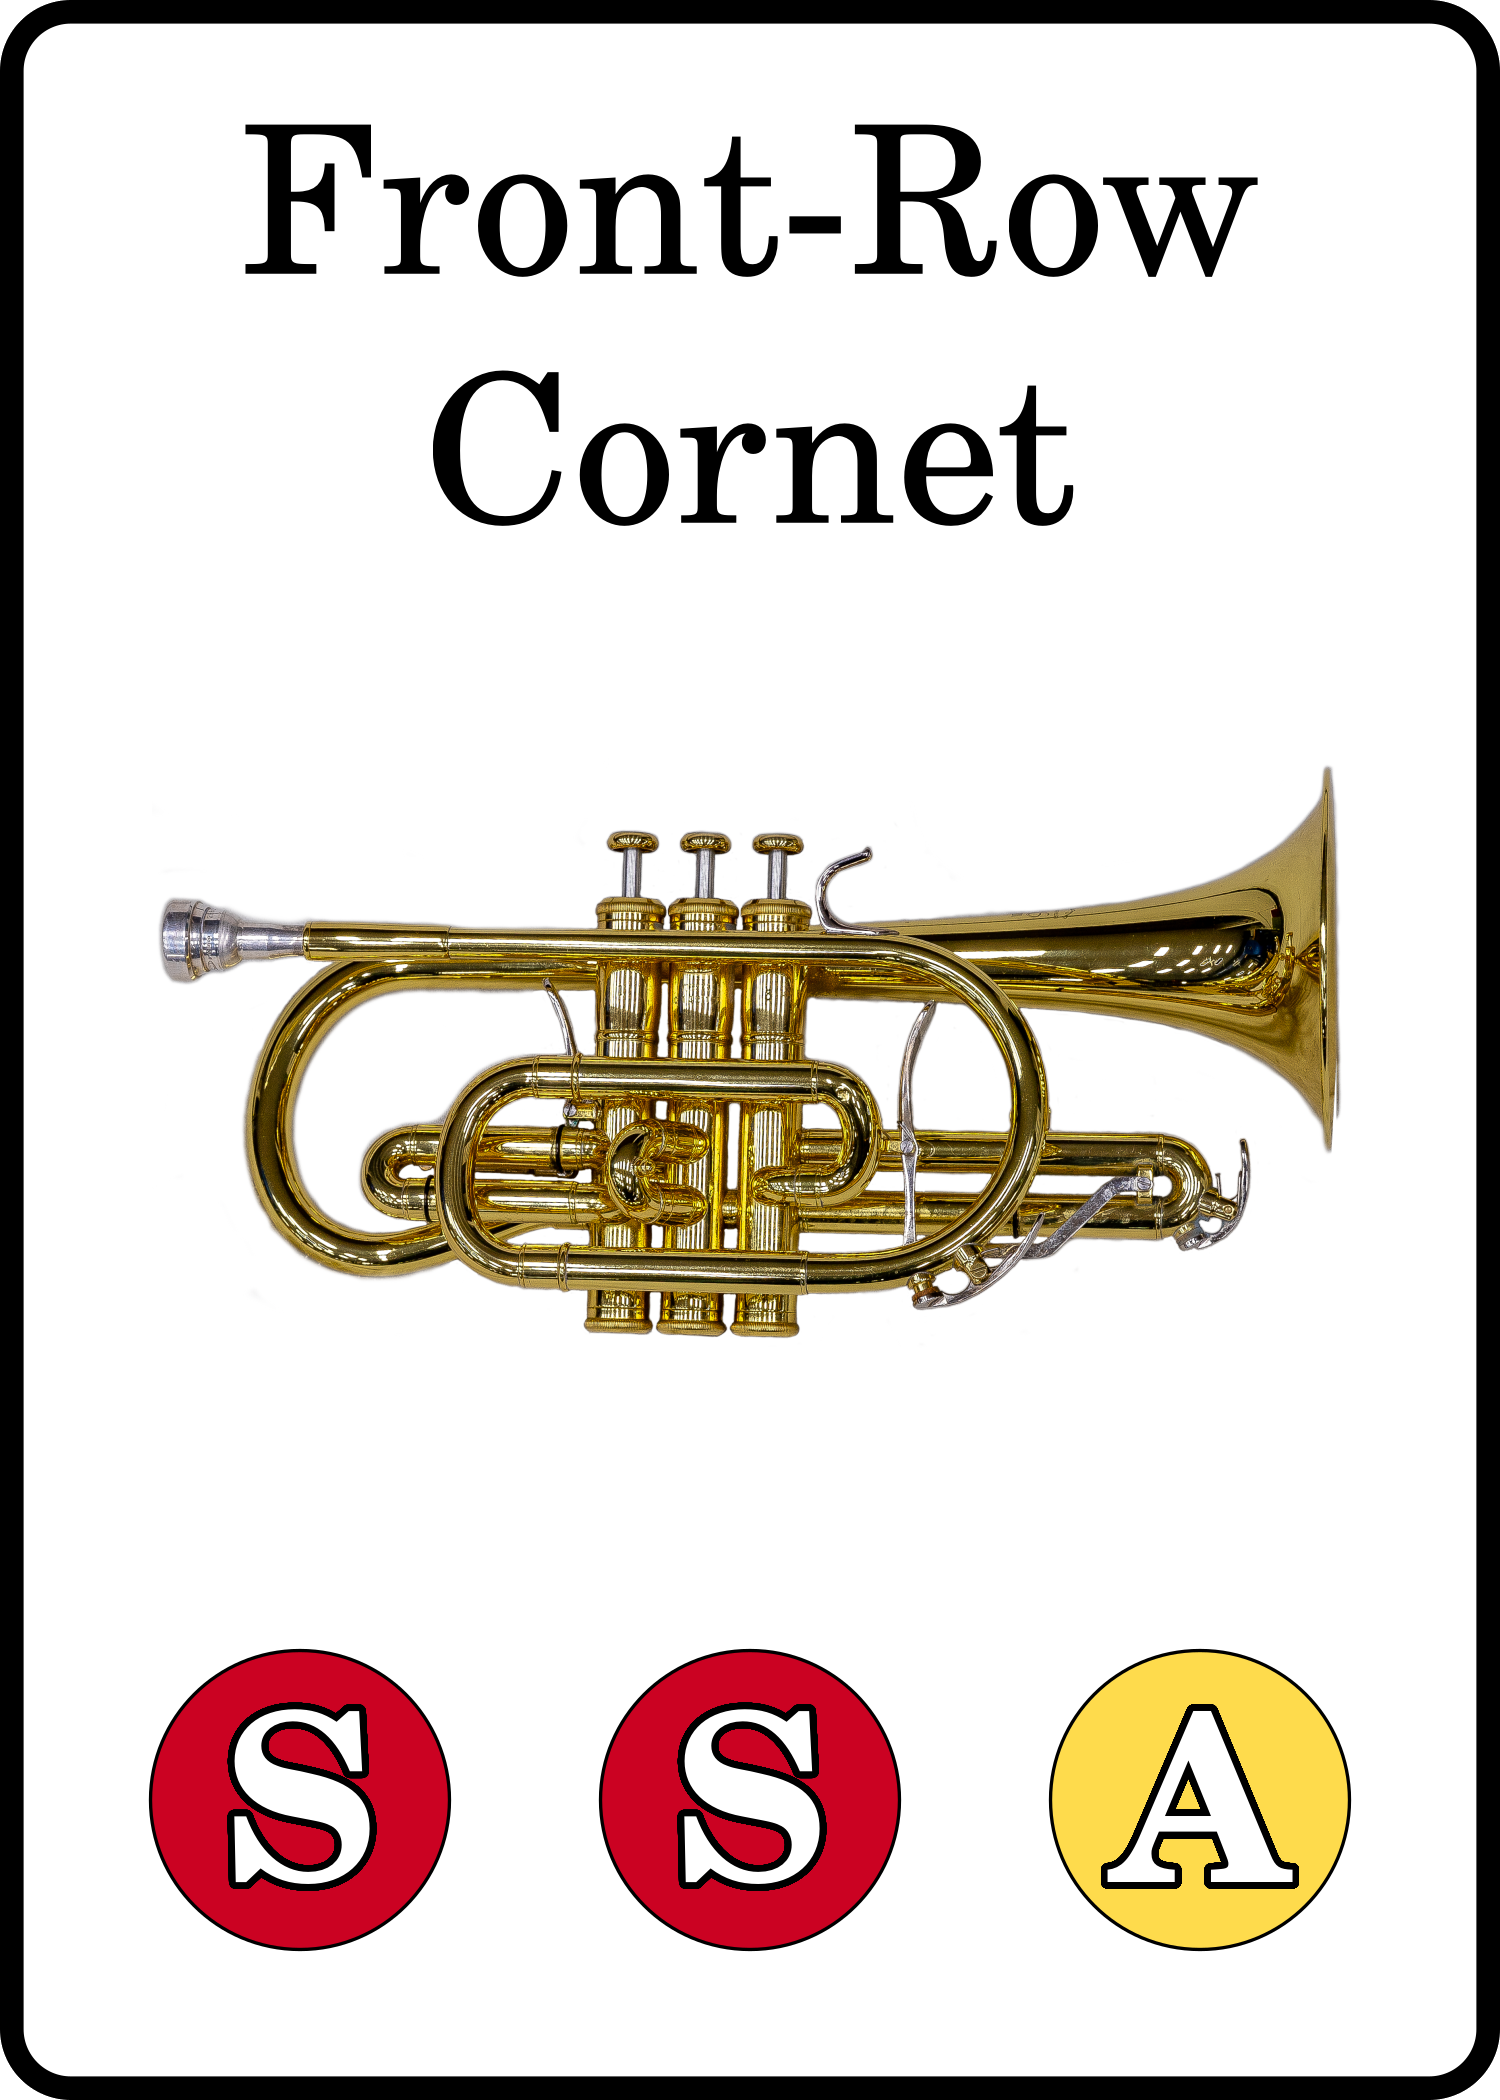
\includegraphics[height=3.75cm]{Images/CardImages/cornet_display_front.png}};

\path (b.south west) --++ (0cm, -5.025cm) node[anchor=north west, rotate=0, transform shape, inner sep=0pt] (s) {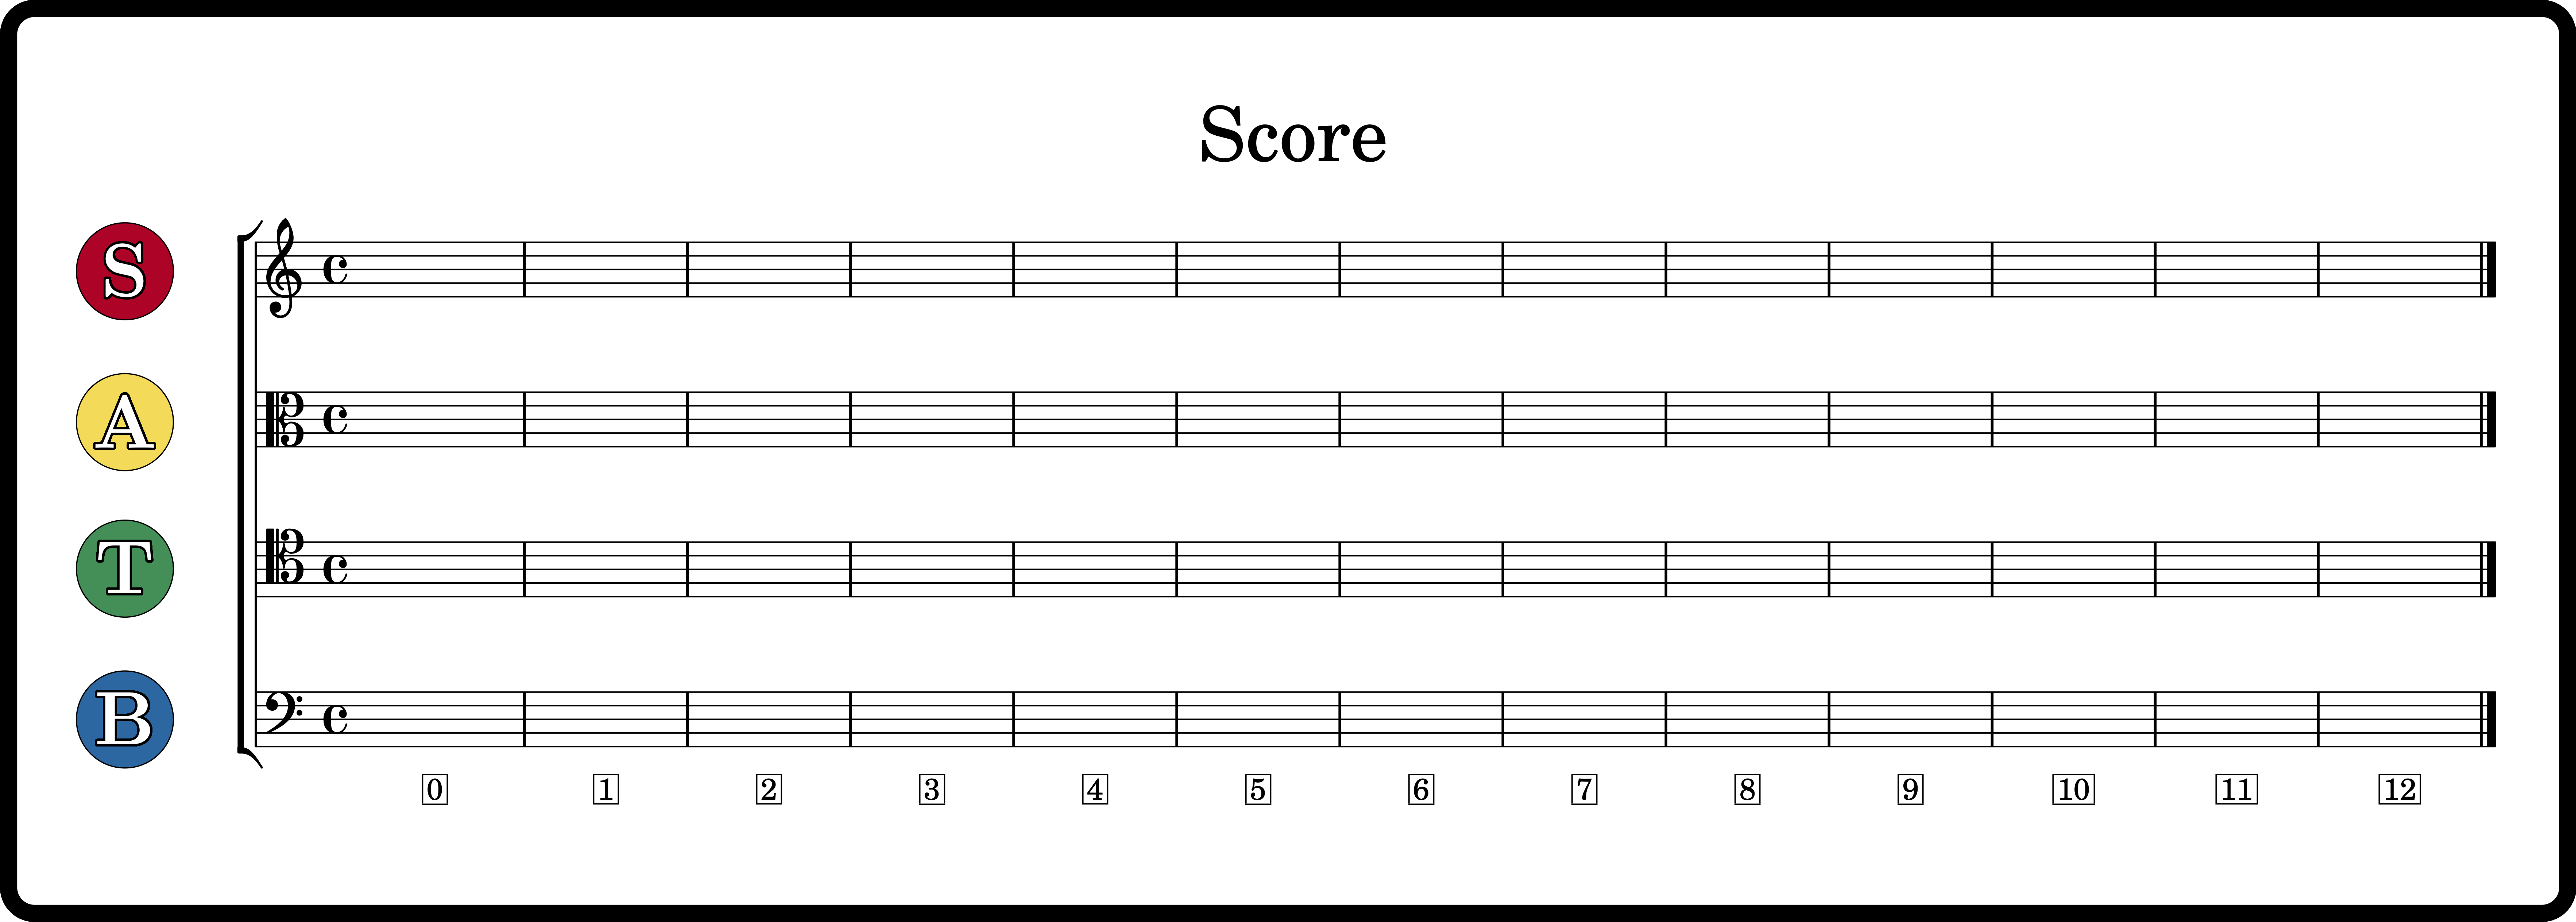
\includegraphics[width=72mm]{Images/score_display_front.png}};


\path (a.south east) --++ (0, -0.5cm) node[draw, line width=0.5mm, text width=50mm, inner sep=5mm, fill=white, fill opacity=0.9, rounded corners=1mm, anchor=north east, text depth=8.7cm] (c) {\vspace{-2ex}\section*{Features} \begin{itemize}[leftmargin=*]
\item Players draft cards to assemble eight different performances.
\item Each performance is evaluated for its merits in four different voices.
\item Only a player's worst voice overall determines their final score.
\item These simple mechanics force players to make difficult choices about the tactical and strategic consequences of each card that they draft.
%\item Tactical decisions with strategic implications.
\end{itemize}
};

\path (s.south west) --++ (0, -0.5cm) node[anchor=north west, text width=62mm, inner sep=4.85mm, draw, line width=0.5mm, fill=white, fill opacity=0.9, rounded corners=1mm] {\textcolor{redfabric}{\textbf{\scshape{Designed By:}}} Michael Purcell\\\textcolor{redfabric}{\textbf{\scshape{Contact:}}} ttkttkt@gmail.com};

\path (c.south west) --++ (0, -0.5cm) node[anchor=north west, inner sep=2mm, draw, line width=0.5mm, fill=white, fill opacity=0.9, rounded corners=1mm, minimum width=1.25cm] {\tikz{
\node[inner sep=0pt] (pc) {
\includegraphics[scale=0.125]{Images/Icons/player_count_icon_red.png}};
\path (pc.south west) --++ (0, 0.08cm) node[inner sep=0pt] {\textcolor{redfabric}{\textbf{2}}};
}};

\path (c.south) --++ (0, -0.5cm) node[anchor=north, inner sep=2mm, draw, line width=0.5mm, fill=white, fill opacity=0.9, rounded corners=1mm, minimum width=1.25cm] {\tikz{
\node[inner sep=0pt] (pc) {
\includegraphics[scale=0.125]{Images/Icons/play_time_icon_red.png}};
\path (pc.south) --++ (0, 0.08cm) node[inner sep=0pt] {\textcolor{redfabric}{\textbf{20-30}}};
}};

\path (c.south east) --++ (0, -0.5cm) node[anchor=north east, inner sep=2mm, draw, line width=0.5mm, fill=white, fill opacity=0.9, rounded corners=1mm, minimum width=1.25cm] {\tikz{
\node[inner sep=0pt] (pc) {
\includegraphics[scale=0.125]{Images/Icons/player_age_icon_red.png}};
\path (pc.south east) --++ (0, 0.08cm) node[inner sep=0pt] {\textcolor{redfabric}{\textbf{12+}}};
}};
\end{tikzpicture}

\end{document}